%
% fig-loxodrome.tex
%
% (c) 2025 Prof Dr Andreas Müller
%
\begin{figure}
\centering
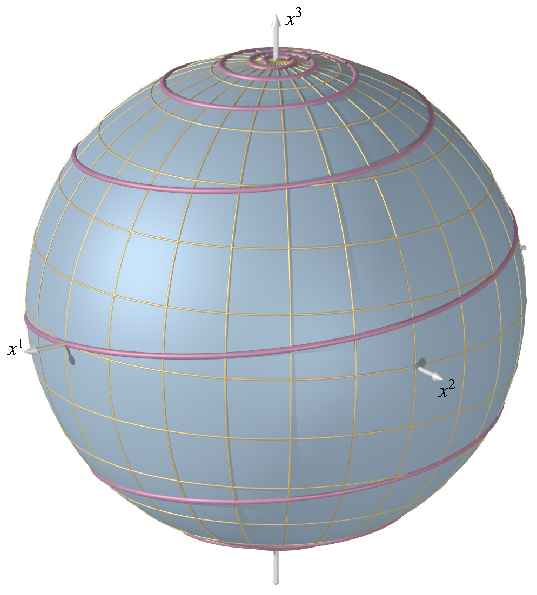
\includegraphics{chapters/030-kurvenintegral/images/loxodrome.pdf}
\caption{Die Loxodrome auf einer Kugeloberfläche schneidet die Längen- und
Breitenkreise unter konstantem Winkel.
Als Abbildung $\mathbb{R}\to S^2$ transportiert die Loxodrome die
$1$-Form $\sin^2\vartheta\,d\varphi$ auf der Kugeloberfläche auf die
reelle Achse und macht daraus die $1$-Form $(1-\tanh^2 kt)\,dt$.
\label{buch:kurvenintegral:fig:loxodrome}}
\end{figure}
